\section{Qualitative Results}
\label{sec:qualitative-results}


  \begin{figure}[h]
    \centering
    \fbox{\parbox{0.7\textwidth}{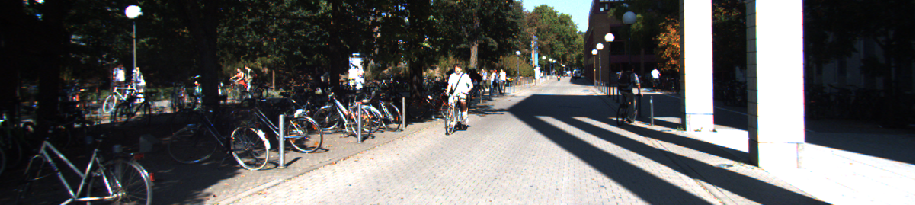
\includegraphics[width=\linewidth]{visual_results/rgb1}
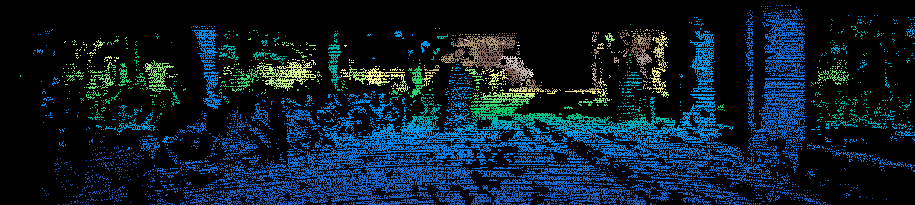
\includegraphics[width=\linewidth]{visual_results/ground1}
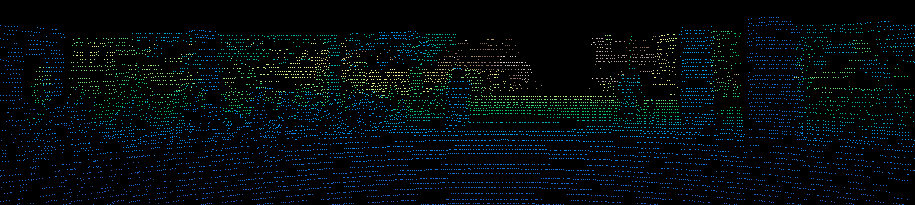
\includegraphics[width=\linewidth]{visual_results/input1}
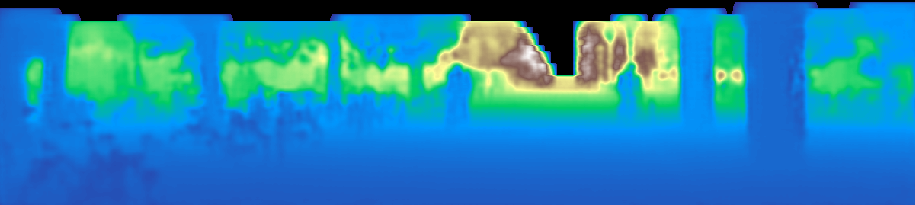
\includegraphics[width=\linewidth]{visual_results/prediction1}}}
\caption{KITTI Sample Output. From top to bottom: RGB Image, ground truth, input prediction}
\label{fig:vis1}
\end{figure}

\begin{figure}[h]
  \centering
  \fbox{\parbox{0.7\textwidth}{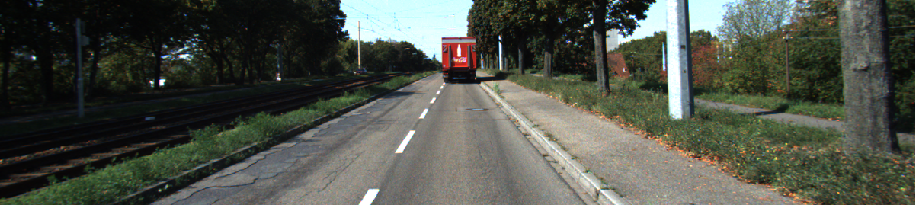
\includegraphics[width=\linewidth]{visual_results/rgb2}
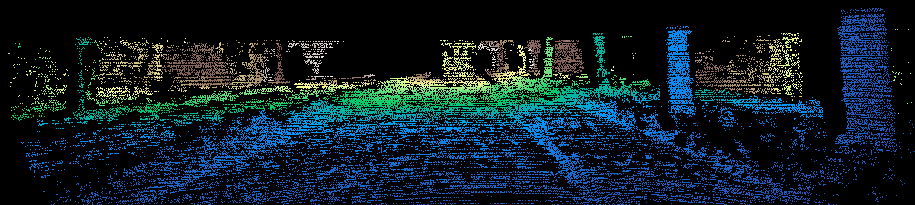
\includegraphics[width=\linewidth]{visual_results/ground2}
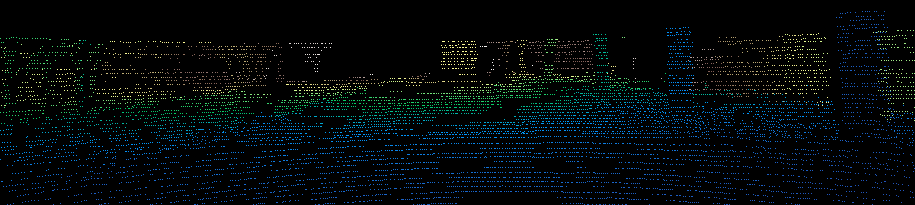
\includegraphics[width=\linewidth]{visual_results/input2}
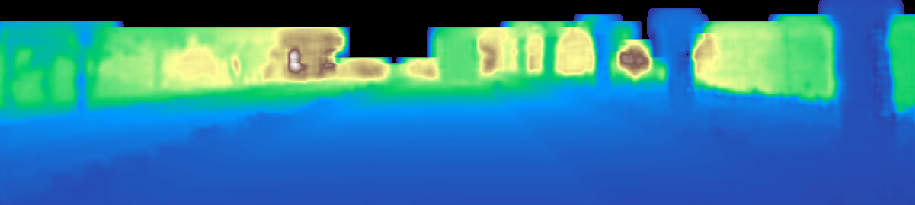
\includegraphics[width=\linewidth]{visual_results/prediction2}}}
\caption{KITTI Sample Output. From top to bottom: RGB Image, ground truth, input prediction}
\label{fig:vis2}
\end{figure}

\begin{figure}[h]
  \centering
  \fbox{\parbox{0.7\textwidth}{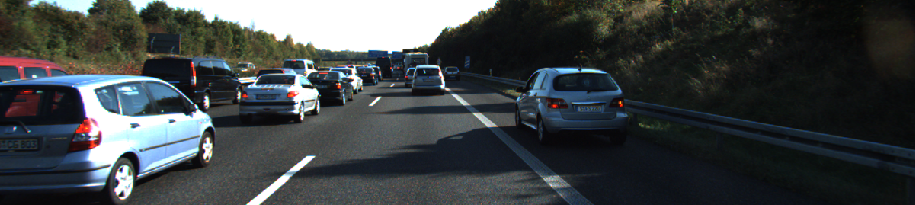
\includegraphics[width=\linewidth]{visual_results/rgb3}
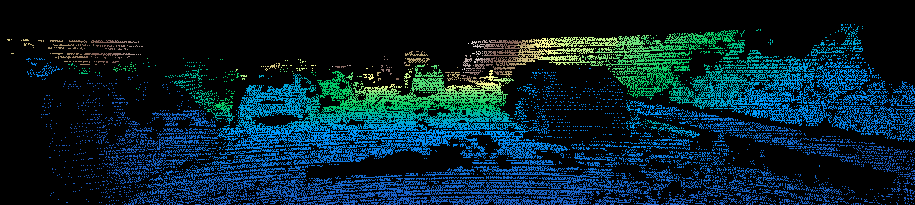
\includegraphics[width=\linewidth]{visual_results/ground3}
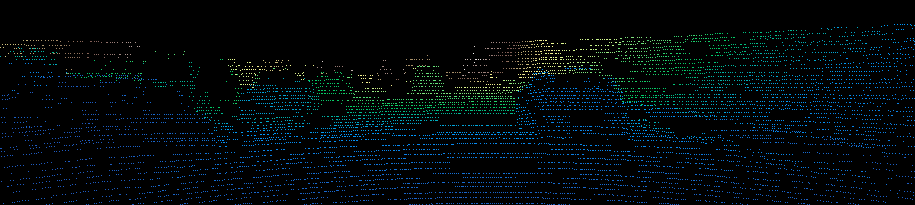
\includegraphics[width=\linewidth]{visual_results/input3}
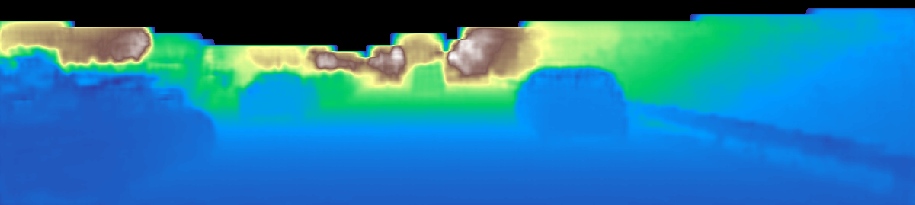
\includegraphics[width=\linewidth]{visual_results/prediction3}}}
\caption{KITTI Sample Output. From top to bottom: RGB Image, ground truth, input prediction}
\label{fig:vis3}
\end{figure}

